\documentclass[aspectratio=169,11pt]{beamer}

\usetheme{Madrid}
\usecolortheme{default}
\usefonttheme{professionalfonts}
\setbeamertemplate{navigation symbols}{}
\setbeamertemplate{footline}[frame number]

\usepackage{amsmath, amssymb, booktabs, graphicx}
\graphicspath{{../../assets/figures/}{assets/figures/}}

\title{Human Capital and Skill Formation}
\subtitle{Labor I --- Week 4}
\author{Teaching deck draft}
\date{}

\begin{document}

\begin{frame}
  \titlepage
\end{frame}

\begin{frame}{Central question and motivation}
\begin{itemize}
    \item Week 3 asked how workers time labor supply given productive capacity.
    \item Week 4 asks where productive capacity comes from.
    \item Schooling, training, and childhood investments are all versions of the same dynamic tradeoff: pay now, produce later.
\end{itemize}
\end{frame}

\begin{frame}{Why Week 3 is not enough}
\begin{itemize}
    \item Dynamic labor supply treats wages as moving objects, but it does not yet explain why wages rise over the lifecycle.
    \item Observed age-earnings profiles reflect accumulated skill, not only changing prices or preferences.
    \item We need an explicit state variable for productive capacity before we can interpret returns to skill.
\end{itemize}
\end{frame}

\begin{frame}{Ben-Porath law of motion}
\[
h_{t+1} = (1-\delta_h) h_t + A_t i_t^{\alpha},
\qquad
w_t = r_t h_t
\]

\begin{itemize}
    \item Human capital is a state variable.
    \item Current investment raises future wages through future productivity.
    \item Remaining work horizon is what makes early investment especially valuable.
\end{itemize}
\end{frame}

\begin{frame}{Investment tradeoff}
\[
\text{MC}_t(i_t)
=
\beta \, \mathbb{E}_t
\left[
\sum_{s=t+1}^{T}
\beta^{s-t-1}
\frac{\partial w_s}{\partial h_s}
\frac{\partial h_s}{\partial i_t}
\right]
\]

\begin{itemize}
    \item The cost side is tuition, effort, and foregone earnings.
    \item The benefit side is the discounted stream of higher future productivity.
    \item This is why lifecycle wage growth and schooling choice belong in one framework.
\end{itemize}
\end{frame}

\begin{frame}{Lifecycle human capital and earnings}
\begin{center}
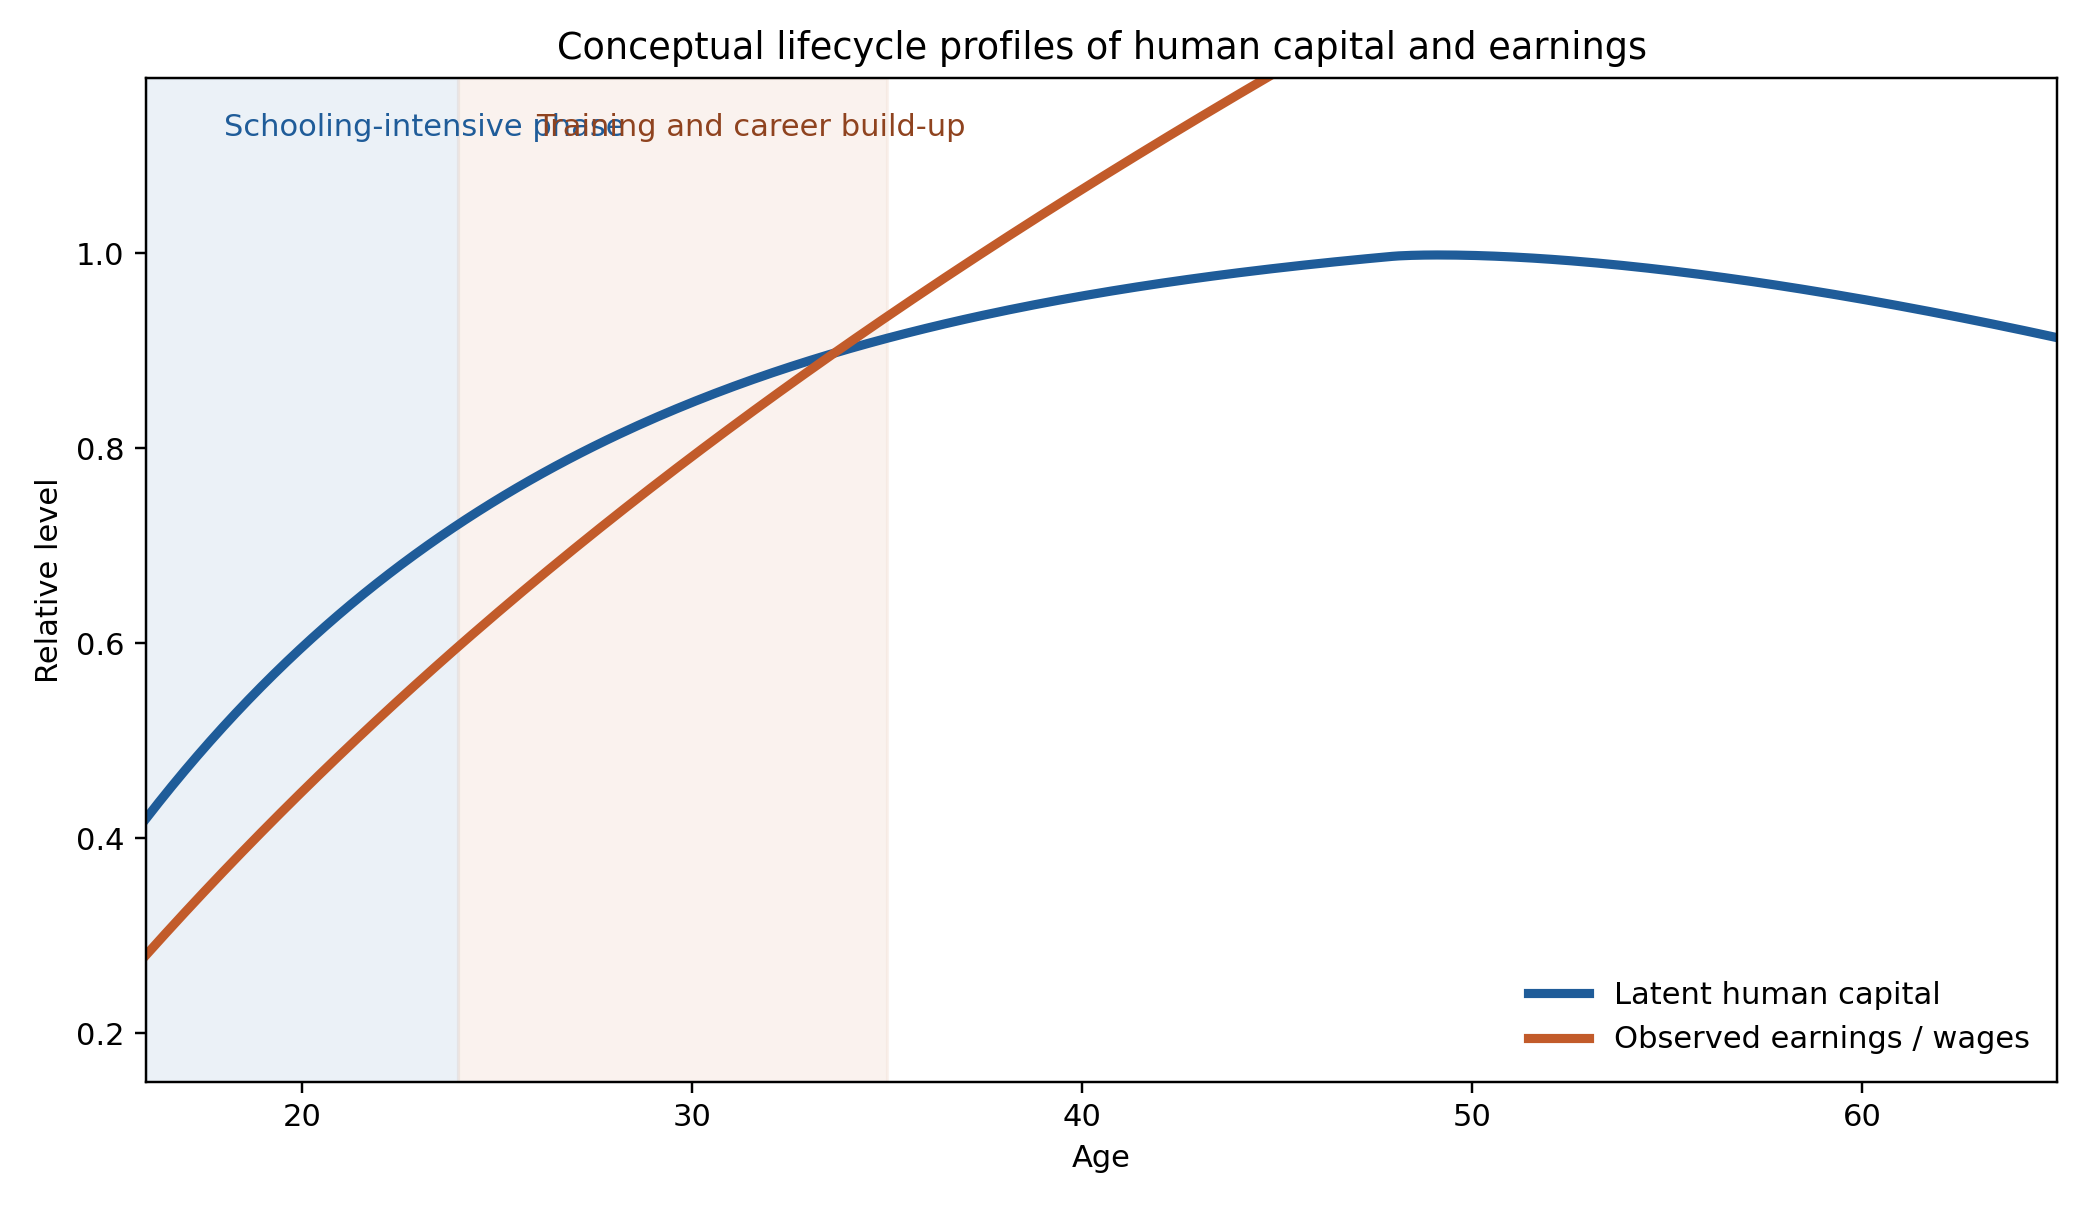
\includegraphics[height=0.74\textheight,keepaspectratio]{04-lifecycle-human-capital-earnings.png}
\end{center}
\end{frame}

\begin{frame}{Schooling versus training as accumulation margins}
\begin{center}
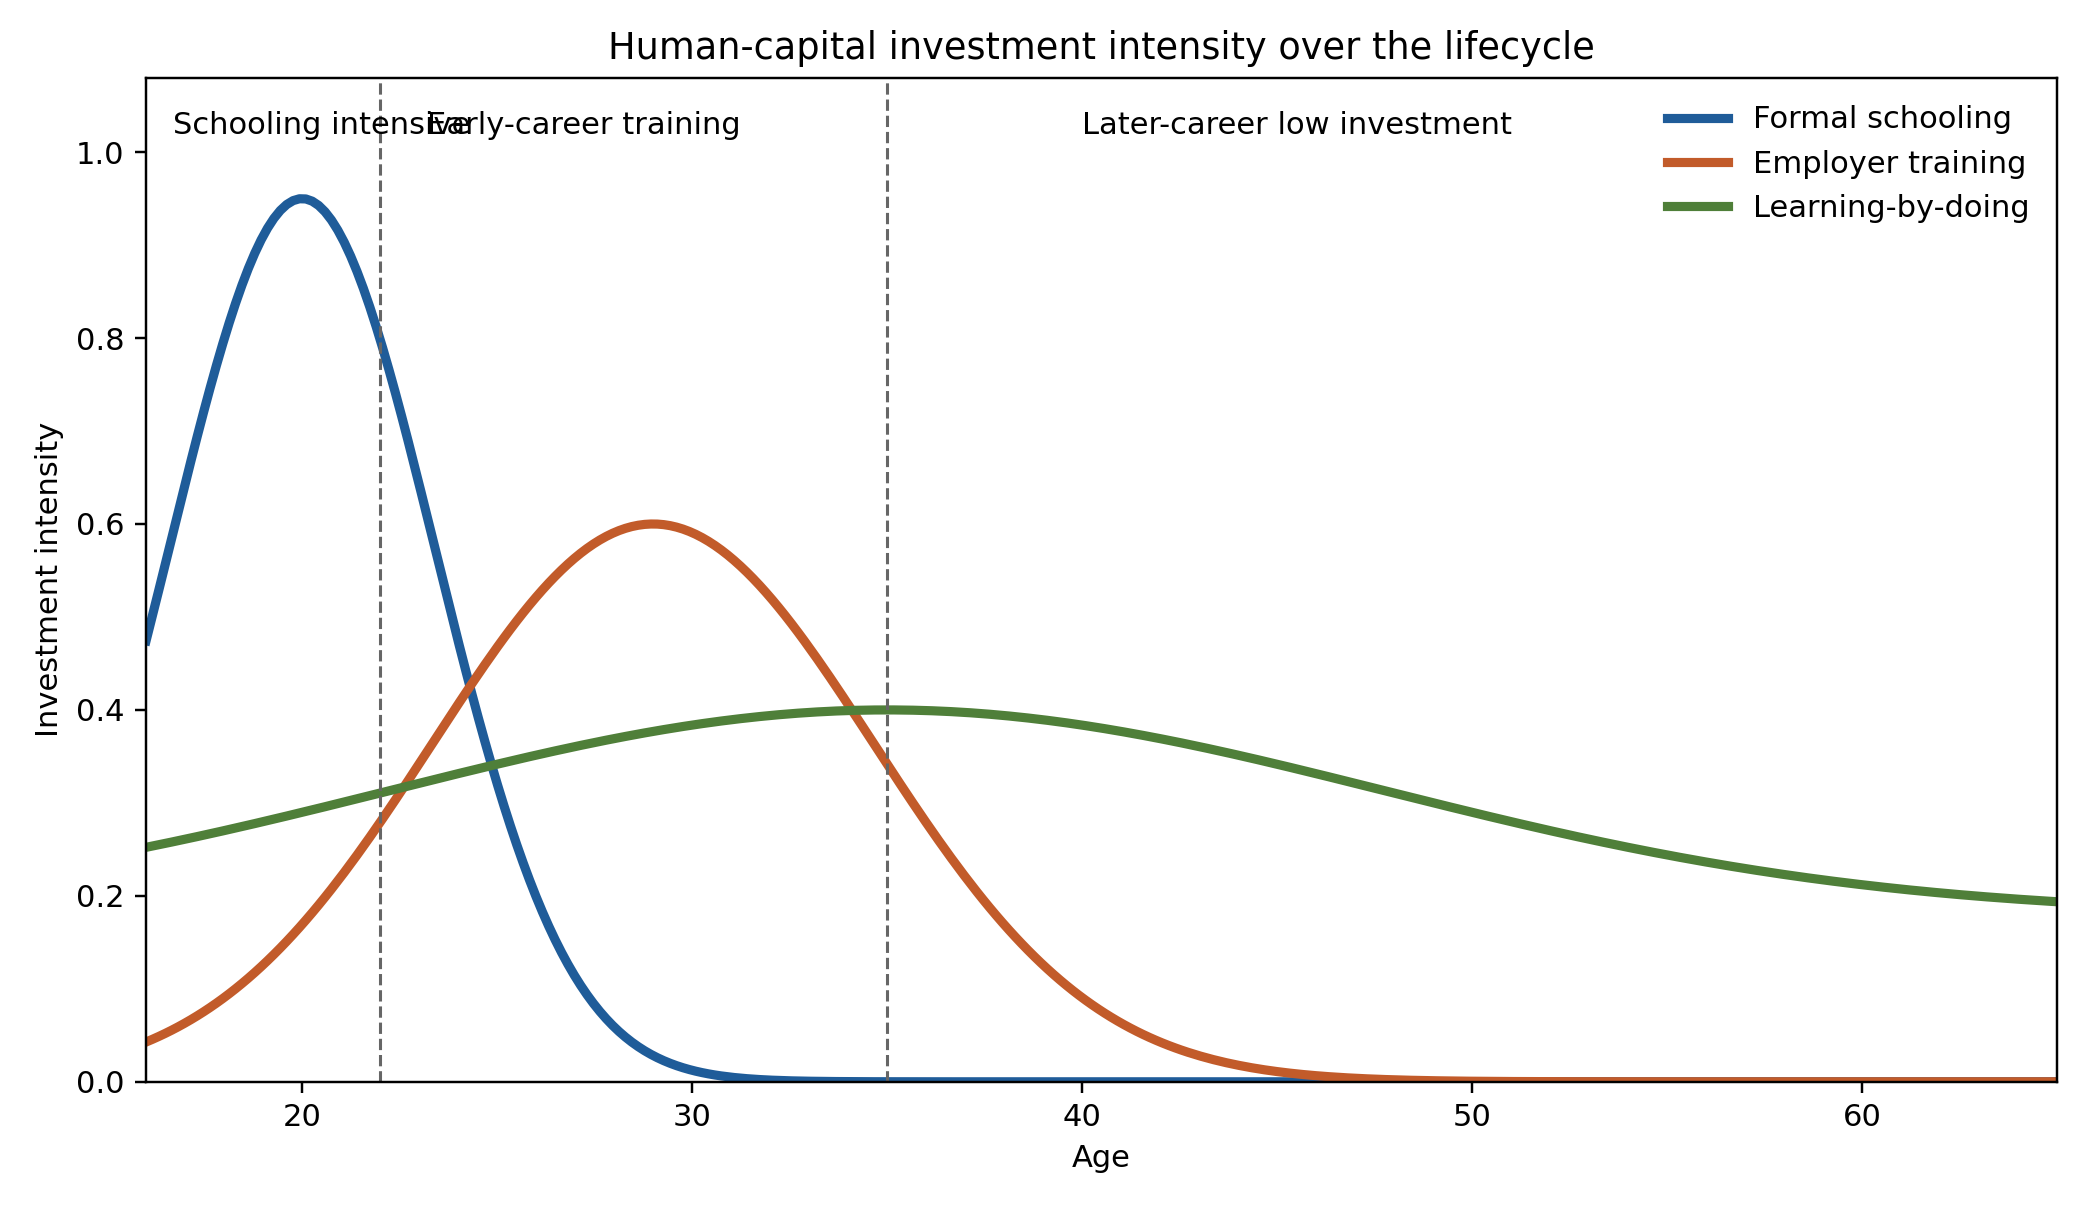
\includegraphics[height=0.74\textheight,keepaspectratio]{04-investment-intensity-lifecycle.png}
\end{center}
\end{frame}

\begin{frame}{General versus specific training}
\begin{itemize}
    \item Becker benchmark: firms should not pay for transferable general training in frictionless markets.
    \item Imperfect labor markets change the result.
    \item Wage compression, turnover frictions, and monopsony power can make firm-sponsored general training privately profitable.
    \item Training incidence is therefore informative, but not a complete measure of investment.
\end{itemize}
\end{frame}

\begin{frame}{Self-productivity and dynamic complementarity}
\[
\theta_{t+1} = f_t(\theta_t, I_t, P_t)
\]

\begin{itemize}
    \item Self-productivity: current skill directly raises future skill.
    \item Dynamic complementarity: later investment is more productive when earlier skill is higher.
    \item Early environments matter because they change the payoff to later schooling and training.
\end{itemize}
\end{frame}

\begin{frame}{Dynamic complementarity schematic}
\begin{center}
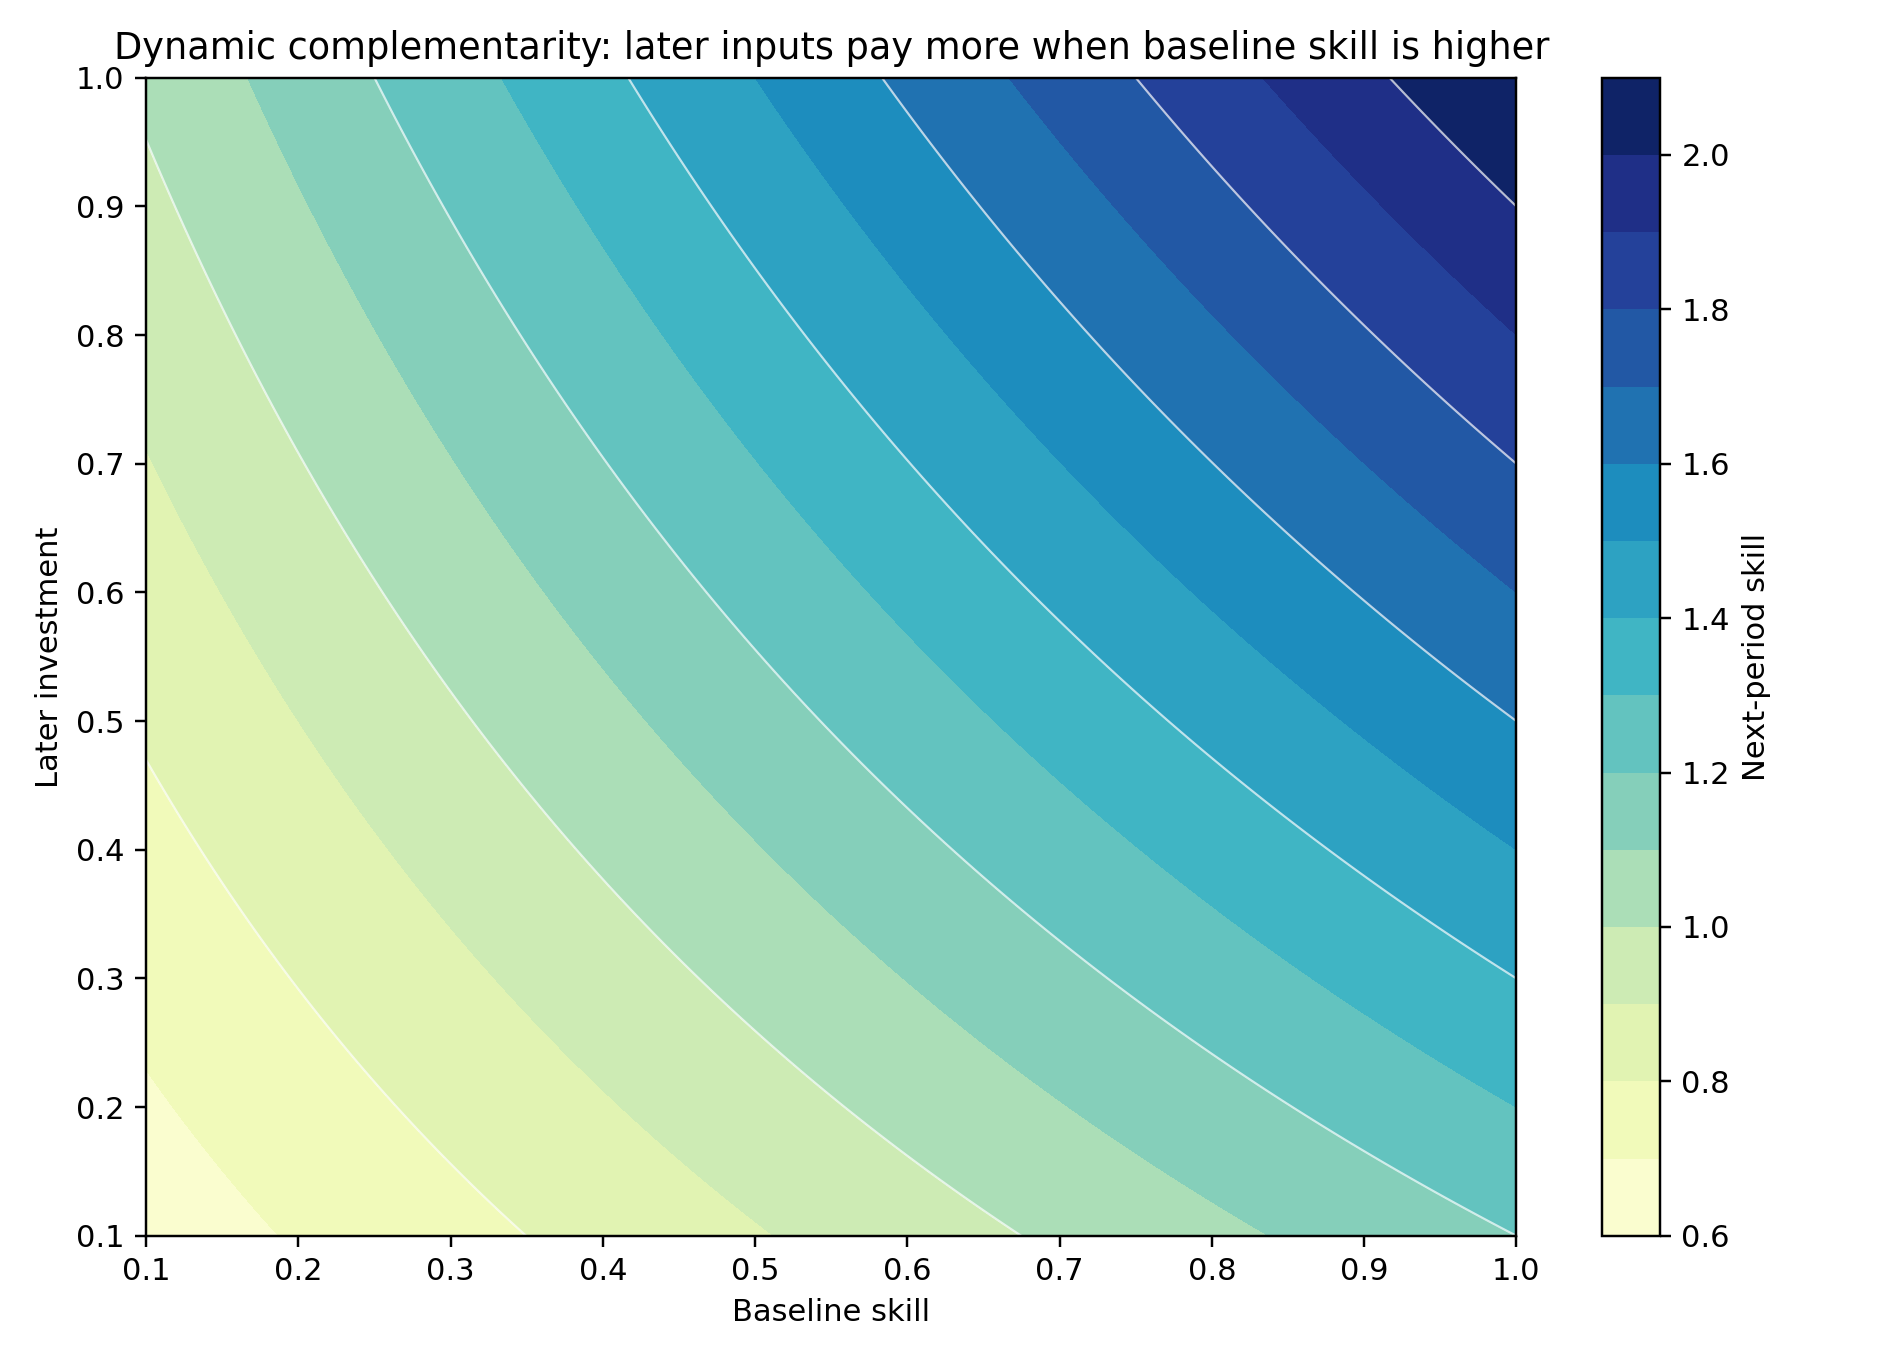
\includegraphics[height=0.72\textheight,keepaspectratio]{04-dynamic-complementarity.png}
\end{center}
\end{frame}

\begin{frame}{Empirical design map}
\small
\begin{tabular}{p{0.24\linewidth} p{0.29\linewidth} p{0.33\linewidth}}
\toprule
Design & Main variation & Object learned \\
\midrule
Schooling subsidy / draft-lottery & Exogenous schooling incentive & Reduced-form return on a narrow margin \\
Randomized childhood intervention & Program-induced input shift & Causal effect of bundled investments \\
Input-composition evidence & Center or input mix differences & Which inputs co-move with gains \\
Structural production function & Modeled skill dynamics & Technology parameters and complementarities \\
Credit-constraint design & Aid or borrowing environment & Whether finance distorts investment \\
\bottomrule
\end{tabular}
\end{frame}

\begin{frame}{Frictions, finance, and policy}
\begin{itemize}
    \item Borrowing constraints and limited commitment can distort high-return schooling investments.
    \item Information frictions change take-up and program choice even when subsidies are unchanged.
    \item Employer-side frictions shape who receives training and who captures the return.
    \item Human-capital policy therefore includes finance, advising, training support, and early-childhood inputs.
\end{itemize}
\end{frame}

\begin{frame}{Core versus extension material}
\begin{itemize}
    \item Core lecture: Ben-Porath, schooling versus training, general versus specific training, self-productivity, design map, policy frictions.
    \item Extension block: deeper production-function estimation and schooling-finance models.
    \item Lab path: bounded synthetic reproduction in the spirit of Attanasio et al., then a quality-heterogeneity transfer in the spirit of Walters.
\end{itemize}
\end{frame}

\begin{frame}{Bridge to Week 5}
\begin{itemize}
    \item Week 4 explains how skill is accumulated.
    \item Week 5 asks how labor markets price that skill.
    \item Observed wage returns mix human-capital accumulation, selection, and wage-setting.
\end{itemize}
\end{frame}

\begin{frame}{Takeaways}
\begin{itemize}
    \item Human capital is a lifecycle state variable, not a fixed trait.
    \item Schooling, training, and childhood investment are different margins of the same dynamic problem.
    \item Early inputs matter partly because they raise the payoff to later inputs.
    \item Finance and information frictions can distort efficient investment and widen inequality.
\end{itemize}
\end{frame}

\appendix

\begin{frame}{Appendix: production-function extension}
\begin{itemize}
    \item Randomized interventions can identify treatment effects without identifying the full production technology.
    \item Structural estimation adds measurement and functional-form assumptions to recover self-productivity and complementarity.
    \item This is the natural extension slide if the class wants the full Attanasio et al. production-function discussion.
\end{itemize}
\end{frame}

\begin{frame}{Appendix: schooling finance extension}
\begin{itemize}
    \item Credit frictions are not only low cash-on-hand.
    \item The key objects are collateral, limited commitment, repayment risk, and when returns arrive.
    \item This is the natural extension slide if the class wants the Lochner--Monge-Naranjo policy bridge.
\end{itemize}
\end{frame}

\end{document}
